% Generated 2021-01-06 15:42:26 +0530
\subsection{Motion} \label{sec:Motion}


\begin{figure}[ht]
  \centering
    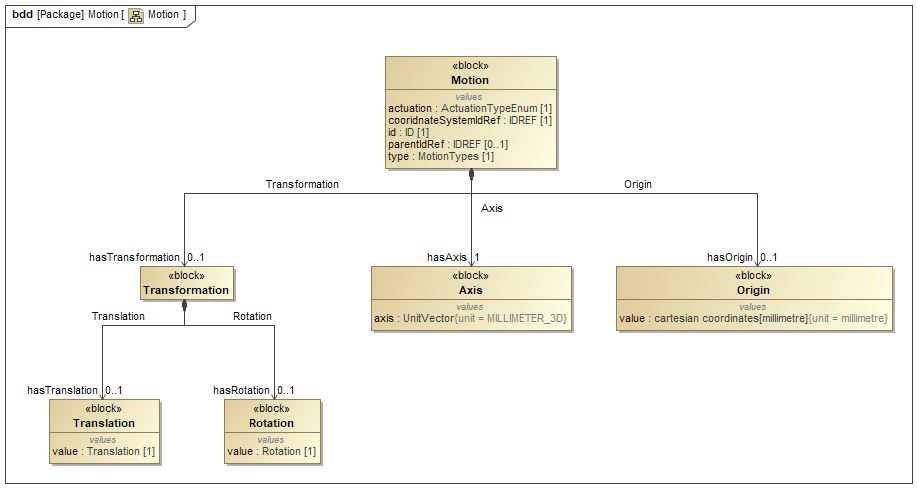
\includegraphics[width=1.0\textwidth]{figures/Motion.png}
  \caption{Motion Diagram}
  \label{fig:Motion}
\end{figure}

\FloatBarrier



\subsubsection{Axis}




\block{Axis} defines the axis along or around which the component moves relative to a coordinate system.


The value of \texttt{Axis} \MUST be \texttt{UnitVector}.


\subsubsection{Motion}
\label{sec:Motion}



\block{Motion} defines the movement of the component relative to a coordinate system. \block{Motion} specifies the kinematic chain of the components.


\paragraph{Attributes of Motion}\mbox{}
\label{sec:Attributes of Motion}

\tbl{Attributes of Motion} lists the attributes of \texttt{Motion}.

\begin{table}[ht]
\centering 
  \caption{Attributes of Motion}
  \label{table:Attributes of Motion}
\tabulinesep=3pt
\begin{tabu} to 6in {|l|l|l|} \everyrow{\hline}
\hline
\rowfont\bfseries {Attribute} & {Type} & {Multiplicity} \\
\tabucline[1.5pt]{}

\property{actuation}[Motion] & \texttt{MotionActuationTypeEnum} & 1 \\
\property{cooridnateSystemIdRef}[Motion] & \texttt{IDREF} & 1 \\
\property{id}[Motion] & \texttt{ID} & 1 \\
\property{parentIdRef}[Motion] & \texttt{IDREF} & 0..1 \\
\property{type}[Motion] & \texttt{MotionTypes} & 1 \\
\end{tabu}
\end{table}
\FloatBarrier

Descriptions for attributes of \block{Motion}:

\begin{itemize}

\item \property{actuation}[Motion] \newline Describes if this component is actuated directly or indirectly as a result of other motion.

\texttt{MotionActuationTypeEnum} Enumeration:

\begin{itemize}
\item \texttt{DIRECT} \newline The movement is initiated by the component. 
\item \texttt{VIRTUAL} \newline The motion is computed and is used for expressing an imaginary movement. 
\item \texttt{NONE} \newline There is no actuation of this Axis. 
\end{itemize}


\item \property{cooridnateSystemIdRef}[Motion] \newline The coordinate system within which the kinematic motion occurs.

\item \property{id}[Motion] \newline The identifier of this element.

\item \property{parentIdRef}[Motion] \newline The kinematic chain connects all components using the parent relations. All motion is connected to the motion of the parent. The first node in the chain will not have a parent.

\item \property{type}[Motion] \newline Describes the type of motion.

\texttt{MotionTypes} Enumeration:

\begin{itemize}
\item \texttt{PRISMATIC} \newline Sliding linear motion along an axis with a fixed range of motion. 
\item \texttt{CONTINUOUS} \newline Revolves around an axis with a continuous range of motion. 
\item \texttt{REVOLUTE} \newline Rotates around an axis with a fixed range of motion. 
\item \texttt{FIXED} \newline The axis does not move. 
\end{itemize}

\end{itemize}

\paragraph{Elements of Motion}\mbox{}
\label{sec:Elements of Motion}

\tbl{Elements of Motion} lists the elements of \texttt{Motion}.

\begin{table}[ht]
\centering 
  \caption{Elements of Motion}
  \label{table:Elements of Motion}
\tabulinesep=3pt
\begin{tabu} to 6in {|l|l|} \everyrow{\hline}
\hline
\rowfont\bfseries {Element} & {Multiplicity} \\
\tabucline[1.5pt]{}
\texttt{Axis} & 0..1 \\
\texttt{Origin} & 0..1 \\
\texttt{Transformation} & 0..1 \\
\texttt{Description} & 0..1 \\
\end{tabu}
\end{table}
\FloatBarrier


Descriptions for elements of \block{Motion}:

\begin{itemize}

\item \block{Axis} \newline \block{Axis} defines the axis along or around which the component moves relative to a coordinate system.

\item \block{Origin} \newline A fixed point from which measurement or motion commences.

\item \block{Transformation} \newline The transformation of the parent \block{Origin} or \block{Transformation} using \block{Translation} and \block{Rotation}. At a minimum, a \block{Translation} or \block{Rotation} \textbf{MUST} be given.

\item \block{Description} \newline The descriptive content.
\end{itemize}
